\section{Valid Inequalities}
\label{sec:valid_inequalities}

\paragraph{} To investigate the integrality properties of the model, we initially relaxed the binary constraints and solved the resulting linear programming formulation. This preliminary analysis was conducted on simple graph instances, beginning with a tree consisting of three nodes, as illustrated in \textsl{\autoref{fig:tree3}}. The relaxed problem was solved for $k=2$, and the solution obtained was fractional as shown below.

\begin{figure}[H]
    \centering
    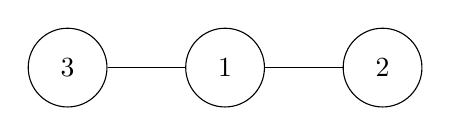
\begin{tikzpicture}[every node/.style={circle, draw, minimum size=1cm}]
  \node (v1) at (0,0) {3};
  \node (v2) at (2,0) {1};
  \node (v3) at (4,0) {2};

  \draw (v1) -- (v2) -- (v3);
\end{tikzpicture}
    \caption{The tree with 3 nodes to be solved}
    \label{fig:tree3}
\end{figure}

\[
\begin{array}{c@{\hskip 2cm}c}
\textbf{x} = 
\begin{pmatrix}
x_{1,1} \\
x_{2,1} \\
x_{3,1} \\
x_{1,2} \\
x_{2,2} \\
x_{3,2}
\end{pmatrix}
=
\begin{pmatrix}
0 \\
1.0 \\
0.5 \\
1.0 \\
0 \\
0.5
\end{pmatrix}
&
\textbf{d} = 
\begin{pmatrix}
d_{1,1} \\
d_{2,1} \\
d_{3,1} \\
d_{1,2} \\
d_{2,2} \\
d_{3,2}
\end{pmatrix}
=
\begin{pmatrix}
1.0 \\
0.5 \\
0 \\
0 \\
0.5 \\
1.0
\end{pmatrix}
\end{array}
\]

\paragraph{} Subsequently, we aimed to strengthen the formulation by introducing a valid inequality intended to eliminate the observed fractional solution and better approximate the convex hull of the feasible integer region. Through this process, we derived the valid inequality:

\begin{equation}
    \sum_{v \in V} x_{v,1} \geq \left\lceil \frac{|V|}{k} \right\rceil \label{eq:valid1}
\end{equation}

where $|V|$ denotes the total number of vertices and $k$ is the number of partitions. The rationale behind this valid inequality is to ensure that the number of vertices assigned to the first partition—which is expected to contain the most due to the ordering assignment constraints—is not below the average number of vertices per partition. To illustrate the effect of this valid inequality, consider the previously obtained fractional solution in which
\[
x_{2,1} = 1.0, \qquad x_{3,1} = 0.5, \qquad x_{1,2} = 1.0, \qquad x_{3,2} = 0.5.
\]
Here, the sum of assignments to the first partition is
\[
\sum_{v \in V} x_{v,1} = 1.0 + 0.5 = 1.5.
\]
For the case where $|V| = 3$ and $K = 2$, the right-hand side of the inequality evaluates to
\[
\left\lceil \frac{3}{2} \right\rceil = 2.
\]

\paragraph{} Since $1.5 < 2$, the aforementioned solution violates the newly introduced constraint, and is thus excluded from the feasible region of the relaxed model.

\paragraph{} As a result of adding the proposed valid inequalities to the model, it was observed that, for $k=2$, the linear programming relaxation produced only integral extreme points. This finding indicates that, for this instance, the convex hull of feasible integer solutions was obtained. A similar result was observed for the same tree structure with $k=3$, where the relaxation again yielded only integral solutions, suggesting that the formulation describes the convex hull in these cases. To reach this conclusion, random weights between -1 and 1 were assigned to the $x$ and $d$ variables, and the model was resolved multiple times under varying objective functions. In all cases, the optimal solutions remained integral.

\paragraph{} Following a similar rationale to the valid inequality \textsl{\eqref{eq:valid1}}, we further strengthened the formulation by introducing an upper bound on the number of vertices assigned to each partition. Specifically, for each $i \in \Pi$, the following valid inequality was added:
\begin{equation}
    \sum_{v \in V} x_{v,i} \leq \left\lfloor \frac{|V| - k + i}{i} \right\rfloor \quad \forall i \in P \label{eq:valid2}
\end{equation}

Here, $|V|$ denotes the number of vertices, $k$ is the number of partitions, and $i$ is the index of the partition under consideration. This constraint ensures that the number of vertices assigned to the $i$-th partition does not exceed the calculated upper bound, thereby eliminating infeasible or overly large assignments in the relaxed model.




\paragraph{} The analysis was then extended to a tree with four nodes, as illustrated in \textsl{\autoref{fig:tree4}}. For $k=2$, the solver returned the following fractional solution:

\begin{figure}[h]
    \centering
    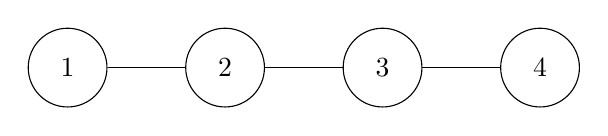
\begin{tikzpicture}[every node/.style={circle, draw, minimum size=1cm}]
  \node (v1) at (0,0) {1};
  \node (v2) at (2,0) {2};
  \node (v3) at (4,0) {3};
  \node (v4) at (6,0) {4};

  \draw (v1) -- (v2) -- (v3) -- (v4);
\end{tikzpicture}
    \caption{The tree with 4 nodes to be solved}
    \label{fig:tree4}
\end{figure}
